\documentclass[a4paper,10pt, english]{report}
\usepackage[T1]{fontenc}
\usepackage[utf8]{inputenc}
\usepackage{babel}
\usepackage{geometry}
\usepackage{graphicx}
\usepackage{amsmath}
\usepackage{booktabs}
\usepackage{url}
\usepackage{longtable}

% Title Page
\title{CMPe 58H - Social Semantic Web\newline Project Report\newline Detecting and analyzing flaming in social media}
\author{Federico Montori}

\begin{document}

\maketitle

\section{Introduction}
Social web and social platforms are currently the most powerful tool to share informations and to express opinions.
Sometimes these opinions can be harmful or simply annoying to other users.
In these cases, the situation can evolve in a real fight made out of comments on comments and sometimes the consequences can be serious (i.e. the tweet posted few weeks ago by Justine Sacco\footnote{http://www.express.co.uk/news/world/450183/IAC-fire-Justine-Sacco-after-racist-tweet-about-trip-to-South-Africa}).
Those fight are what we call ``flames'', according to Wikipedia a ``hostile and insulting interaction between Internet users, often involving the use of profanity'', which are the central element of the project described in this report.
\newline \newline
What we try to do is collect conversations from twitter about ``risky topics'' and indentify which of them actually contain flaming.
After this part we try to perform Social Network Analysis on our results to retrieve some interesting characteristics about the relationships.
\newline \newline 
The project code is available on github at https://github.com/memedum90/TurkuazTurchese-

\section{System overview}
The system is designed as a pipeline of programs and tasks as shown in the picture below.
\begin{figure}[h!]
 \centering
    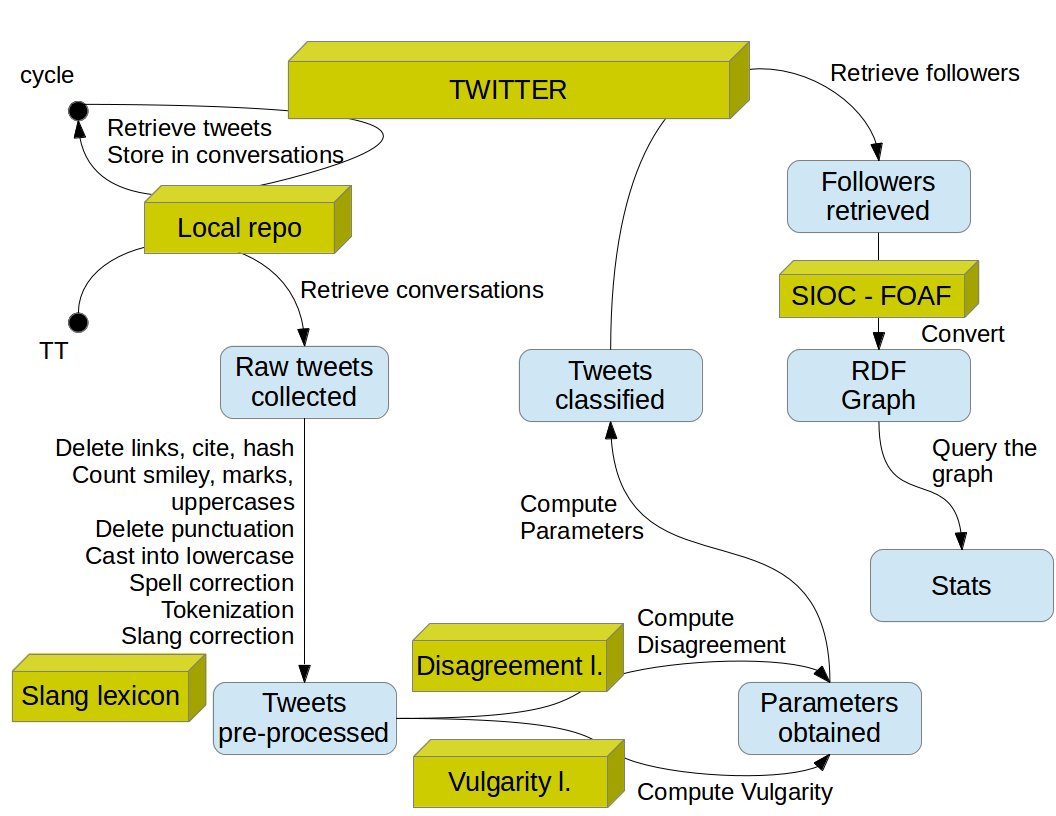
\includegraphics[scale=0.5]{diag1.png}
    \caption{State diagram of the system, including all the external resources.}
\end{figure}


First of all we retrieve tweets and we store them as conversations, as explained in section 3.
Secondly we pre-process the texts contained in the tweets in order to make them readable to our dictionaries and lexicons, as explained in section 4.
Then, we apply our features on all the texts to assign them a ``flaming'' score to decide whether a conversation can be considered as a flame or not.
To evaluate those features we made use of multiple tests on them, as explained in section 5.
\newline
With the results obtained from the previous step, we shift our attention from an NLP task to a SNA task.
Indeed, we convert our users in RDF nodes and the relationships like ``follows'' or ``in a flame'' in object properties, so we can perform multiple SPARQL queries on our resulting graphs.
The idea is that those queries should give us, as an output, some interesting properties made out of statistics in order to come to interesting conclusions.
\newline\newline
To our knowledge this is the very first attempt to try to analyze flames from social networks.
There were some interesting works already performed from which we got some ideas\footnote{Mizil, Sudhof, Jurafsky, Leskovec, Potts - A computational approach to politeness with application to social factors\newline Abu-Jbara, Hassan, Radev - AttitudeMiner: Mining Attitude from Online Discussions\newline Abu-Jbara, Hassan, Radev - Detecting Subgroups in Online Discussions by Modeling Positive and Negative Relations among Participants\newline Ranganath, Jurafsky, McFarland - Detecting friendly, flirtatious, awkward, and assertive speech in speed-dates}.
Despite of these works, we were not able to start from a strong baseline, neither to have some relevant previously annotated data.


\section{Data retrieval}
We retrieved data from twitter simply using the ``tweepy'' python library, so we didn't make use of another ready-to-use tool.
The reason is that, basically, we needed to retrieve conversations, and there is no tool which allows us to do it.
\newline
We chose 15 different topics for our research which are more likely to contain a valuable percentage of flames and debates and less charactierized by sarcasm:
abortion, church, communism, erdogan, euthanasia, feminism,
gaymarriage, gender, holocaust, islamist, jesus, massacre, morsi,
muslim, racism, religion, syria, terrorist.
\newline
The data retrieved has a form of object with multiple fields from which we extracted and renamed the ones we needed:
\begin{itemize}
 \item username: The name of the user who posted, called screen name from the Twitter API
 \item topic: The keyword we user for the research.
 \item user\_id: The ID of the user.
 \item fvt\_cnt: The number of likes that tweet collected.
 \item text: The plain text of the tweet.
 \item reply\_to: The tweet ID for which this tweet is a reply.
 \item rep: Manually added field. The value is 1 if this tweet is a reply, 0 otherwise.
 \item id: Unique ID of the tweet.
 \item rtw\_cnt: Number of retweets of the tweet. 
\end{itemize}
Basically, to retrieve conversations, everytime we obtain a tweet which is a response, we look to the ``reply\_to'' field and extract that tweet too, then we proceed this way until we catch the head of the conversation and we put 0 on the field ``rep''.
This way is easy to collect whole conversations because we have to parse out tweet list and just store a new conversation when we reach the 0.
Of course, due to the twitter API limit, we encountered some problems:
\begin{enumerate}
 \item With a single keyword search we can retrieve about 300 tweets at a time and we have to sleep until the next time window available.
 \item Is given a conversation made out of 3 tweets and structured as follows: $A \to B \to C$ (C is a reply to B, which is a reply to A). If with our keyword we extract B, we can retrieve A, but there's no way in which we can retrieve C.
\end{enumerate}

To perform a proper social network analysis, we needed also another relationship among users, especially we want to know which user follows each other. 
In the first place, we tried to extract all followers and friends of all the authors of at least one post in out dataset, but again Twitter rate limits did not let us do it.
The only solution we could adopt was checking if, for every couple of user in the same conversation, one user is following the other.

\section{Data preprocessing}
To perform our analysis we had to work on the shape of the plain text we retrieved.
To achieve this we work on our data performing the following steps:
 \begin{itemize}
  \item First of all we removed from the plain text every hashtag (word beginning with \#), every citation (word beginning with @) and every hyperlink (word beginning with http://).
  \item We casted everything into lowercase to make our lexicons work homogeneously.
  \item We removed all the puntuation.
  \item We normalized every slang word replacing it with the actual translation. To achieve this, we obtained a huge list of slang terms with the respective meaning from http://noslang.com and we manually modified that.
  \item We checked if the post is actually in english using the guess\_language library, obtained from https://pypi.python.org/pypi/guess-language.
  \item We performed spell correction of a word, checking if the word is in the english dictionary and, if not, substituing it with the closest word in the dictionary if the edit distance is less than 2.
 \end{itemize}

\section{Data features}
In the first place we tried to use the politeness corpus, provided on http://www.mpi-sws.org/~cristian/Politeness.html, as a strong baseline, but we figured out that unfortunately it was not possible because the tweets' texts are too small to performe a proper Naive Bayes evaluation.
So, either to have a good baseline for future work and tobe able to evaluate our performances, we manually annotated more than 2000 tweets, classifying them into two categories (flames or not).
This dataset became our gold standard on which we performed our tests on the features.
The features that we considered were:
\begin{enumerate}
 \item Count of the number of uppercases in a tweet (before casting everything into lowercase). Normally when an user wants to say something strongly and angry is more likely to use uppercases for entire words or even sentences.
 \item Count of the number of question and exclamation marks. In this case, this kind of puntutation is normally repeated when a question or an exclamation is wanted to be stronger by its author.
 \item Count of smiley, bad or good, they are always giving a sense of joke to the whole sentence.
 \item Count of vulgar words, as they are the main characteristic of flames. Normally they can be contained even in other kinds of conversations. The lexicon for vulgar words was manually modified from http://www.cs.cmu.edu/~biglou/resources/bad-words.txt.
 \item Count of co-occurrences between vulgar words and second person singular pronouns like ``you'', ``you're'', ``you'll''. This is more likely to be present more in flames than in other kind of conversations, because it denotes insults directed to the interlocutor.
 \item Count of expressions of disagreement and agreement. We annotated by hand in a lexicon those expressions. Of course, expressions of disagreement like ``that's not true'' are indicators of debate, while the expressions of agreement are the opposite. 
\end{enumerate}
Performing a test, we retrieved the average raw results shown below for flames and not flames conversations:
$$
 \begin{array}{lrr}
 &flames&non-flames\\
 uppercases&44.18&16.70\\
 marks&4.04&1.96\\
 g-smileys&0.18&0.25\\
 b-smileys&0.80&0,57\\
 insults&4.02&0.76\\
 disagreement&0.62&0.24\\
 \end{array}
$$
Applying the proper weights to our features and running our authomatic tool on another manually annotated dataset we achieved the following results:
\begin{itemize}
 \item For flaming we achieved a 0,370 precision, a 0,555 recall and a F-score of 0,0444.
 \item For non-flaming we achieved a 0,913 precision, a 0,833 recall and a F-score of 0,871
\end{itemize}
By our experience we are aware of some well-known bugs. Our method can reach false positives easily when dealing with sarcasm (very difficult to handle), with excess of vulgarity in a common invective (a group of people angry at the same entity) and with too many uppercases in short conversations.
On the other hand we can reach false neagtives when dealing with very long conversations with very short replies.

\section{Social Network Analysis}
After we categorized our conversations in tweets we converted our data in a RDF graph.
First of all, we tried to use as much as we could existing ontologies.
Our users are defined as SIOC entities as well as the relationship sioc:follows, even if it's limited within the conversations.
Every user is linked by a foaf:knows with every other user in the same conversation.
We need to imrove this last definistion, so we designed one further ontology to characterize the fact that a relationship which links users in the same conversations can be a flaming or not and should have a weight.
This weight is the number of tweets belonging to the source user in that conversation.
The picture regarding the graph structure is shown below.
\begin{figure}[h!]
 \centering
    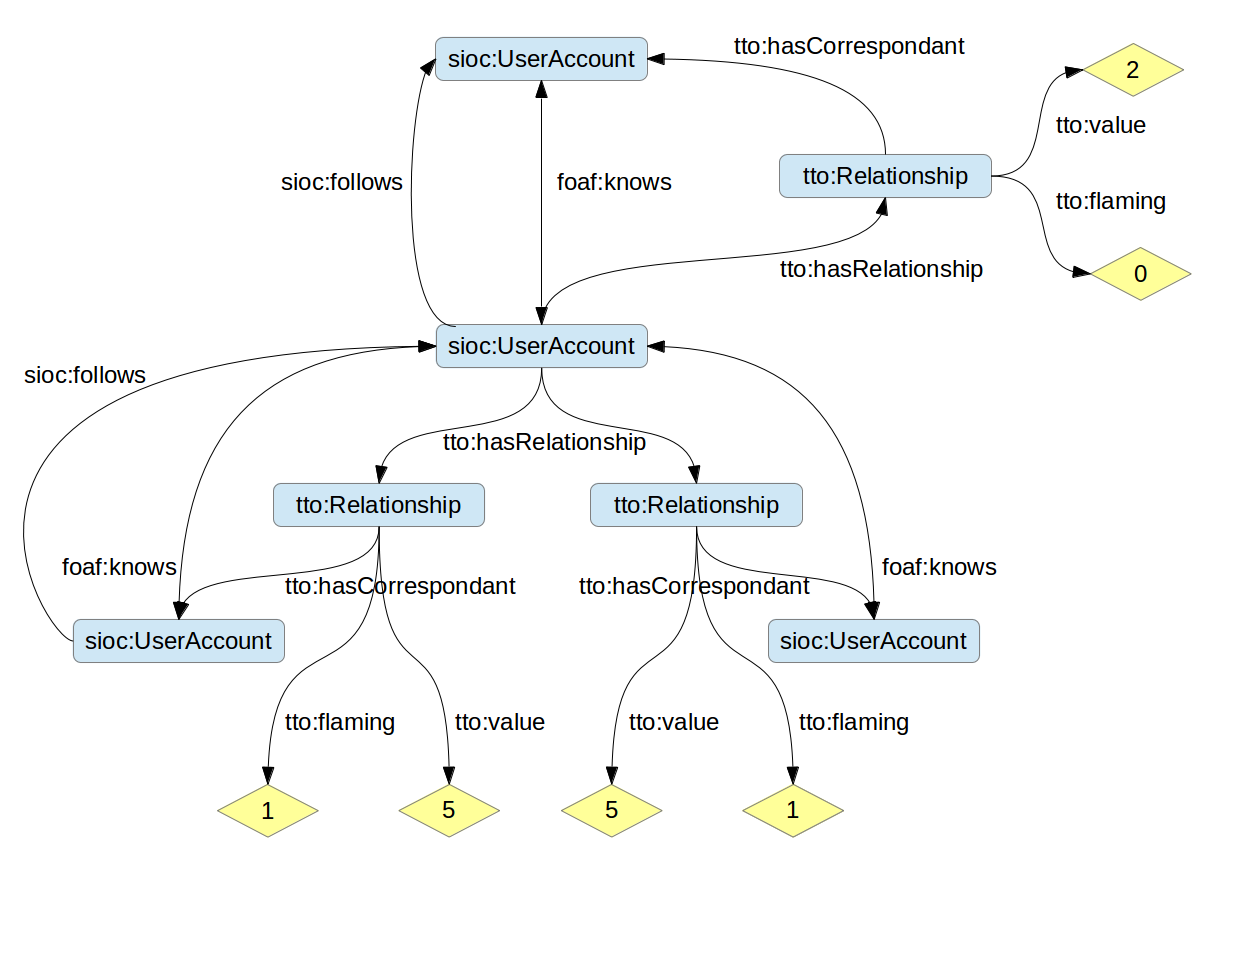
\includegraphics[scale=0.5]{diag2.png}
    \caption{Main use of the ontology.}
\end{figure}
To obtain some values from the SNA we performed the following queries on our RDF graph:
\begin{itemize}
 \item Indegree and outdegree with depth 10. We used the foaf:knows relationship to observe whether a user is a hub (high outdegree, someone who spreads a lot of informations and pposts a lot in multiple domains) or an authority (high indegree, soemone who receives a lot of comments, basically because a lot of users are following him or her).
 \item Indegree and outdegree with depth 1 specifically for flames and not flames. For this property we used our relationship and summed up weights. The purpose of these queries is to understand how much a user is a flamer compared to the number of comversations he is involved in.
 \item Closeness centrality. This measure denotes the capacity of a user to join (and to be reached by) any resource in a network and it's calculated by the inverse sum of its shortest distances to each other resource.
 \item Betweenness centrality. This measure focuses on the capacity of a node to be an intermediary between any two other nodes. It is defined as the ratio between the total number of shortest paths and the number of shortest paths passing though that node.
 \item The last queries we performed are a statistical study on how many time a user A is involved in the same flame as the user B and A follows B or B follows A. We repeated this study on the non-flaming conversations.
 \end{itemize}
Unfortunately, lots of the conversations we retrieved don't have common users with others, so the analysis on betweenness and closeness centrality is not performed correctly.
Surprisingly, our analysis shown that there seems not to be connection between having a flame with someone and following him or her or not.
More specifically, a statistical analysis on our queries gave as result that about in 39\% of cases of couples of users involved in the same flame happens that one user follows the other.
It happens the same for non-flaming conversation: the ratio is about 44\%, not so different from the previous one.
Below are represented the SPARQL queries we performed.

\section{Conclusions and future work}
Due to our dataset, some of our results may seem disappointing, but the most relevant concept is that we developed a baseline for a solid future work.
On the NLP side, annotating manually a huge amount of tweets, we provided a corpus that may be used to perform a Naive Bayes Classification to contribute to our analysis.
On the SSW side, we created a set of useful queries fully working, each one with a specific meaning, so the only improvement should come from a bigger (and more linked) dataset.



\end{document}          
